\documentclass[journal]{IEEEtran}

\usepackage{amsmath}
\usepackage{amsfonts}
\usepackage{amssymb}
\usepackage{amsthm}
%\setcounter{MaxMatrixCols}{20} % needed for wide adjoints

\usepackage{mathdots} % for \iddots

\usepackage{array}

\usepackage{graphicx}

%\usepackage{hyperref}

\newcommand{\opn}[1]{\operatorname{#1}}

%TODO should this be a ``lecture note'' or a ``tips and tricks''?

\begin{document}
%\title{Fast Computation of the Discrete Adjoint Wavelet Transform}
\title{Application of Adjoint Operators in Gradient Computations}
\author{James~Folberth and 
        Stephen~Becker%
\thanks{J. Folberth and S. Becker are with the Department
of Applied Mathematics, University of Colorado at Boulder,
Boulder, CO, 80309 USA}}

\markboth{IEEE Signal Processing Magazine: Lecture Notes}%
{J. Folberth and S. Becker: Fast Adjoint Wavelet}

\maketitle

% For IEEE, Don't use math or other special symbols; greek probably okay.
\begin{abstract}
   When using first-order optimization algorithms, it is often the case that the user must supply the gradient of the differentiable terms in the objective function.  We consider two example problems that have a Euclidean error term involving a linear operation on the problem variables.  The gradient of the Euclidean error term involves both the linear operator and its adjoint, which, in our examples, is not known in the literature.  The first example is an image deblurring problem, where the linear operation is multi-stage wavelet synthesis.  Our formulation of the adjoint holds for a variety of boundary conditions, which allows the formulation to generalize to a larger class of problems.  The second example is a blind channel estimation problem taken from the convex optimization literature; the linear operation is convolution, but with a slight twist.  In each example, we show how the adjoint operator can be applied efficiently.
\end{abstract}

\subsection*{Prerequisites}
The reader should be familiar with linear algebra, wavelets, and basic Fourier analysis.  Knowledge of first-order iterative optimization algorithms is beneficial for motivating the fast adjoint computation, but should not be necessary to understand the adjoint computation itself.  We begin by briefly motivating the need for a fast adjoint operator and then turn toward the two examples.\\


%TODO Not sure what to call this section
%TODO How do we cite Vandenberghe's course notes?
\section{A Model Optimization Problem}
% [[[
In this lecture note we consider as examples a few variants of the standard optimization problem

\begin{equation}
\label{eq:model_problem}
\min_x \frac{1}{2}\|\mathcal{A}x-b\|_2^2 + \lambda \|x\|_1,
\end{equation}

\noindent where $\mathcal{A}$ is a linear operator, $\|\cdot\|_2$ is the $\ell_2$ norm, and $\|\cdot\|_1$ is the $\ell_1$ norm. Let $g(x) = \frac{1}{2}\|\mathcal{A}x-b\|_2^2$ and $h(x)=\lambda \|x\|_1$.  Notice that $g(x)$ is convex and differentiable, and $h(x)$ is convex but non-differentiable.  The scalarization parameter $\lambda$ controls the relative importance of the approximation error $g(x)$ and the sparsity heuristic $\|x\|_1$.  Loosely speaking, larger $\lambda$ should yield a sparser solution.\\

Even though $h(x)$ is non-differentiable, there exist many efficient algorithms for solving the above problem and its variants.  Popular methods include the proximal gradient method and its variants, which include iterative shrinkage thresholding and projected gradient.  Crucial to the speed of these methods is an efficient proximal mapping (prox-operator) for the non-differentiable term $h(x)$.  The proximal mapping is defined as

\[ \opn{prox}_h(x) = \opn{argmin}_{y} \left(h(y) + \dfrac{1}{2}\|y-x\|_2^2\right). \] 

\noindent The proximal mapping can be thought of as finding the point minimizing $h(y)$ plus a simple quadratic model about the point $x$.  For $h(y) = \|y\|_1$, the proximal mapping is the shrinkage (``soft-threshold'') operator and takes the following particularly simple form:

\[ \opn{prox}_h(x) = \left\{\begin{array}{ll} x_i - 1 & x_i \ge 1\\ 0 & |x_i| < 1\\ x_i + 1 & x_i \le 1.\end{array}\right. \]

\noindent The main step of a simple proximal gradient method is

\[ x^{(k)} = \opn{prox}_{t_k h}\left(x^{(k-1)} - t_k \nabla g(x^{(k-1)})\right), \] 

\noindent with step size $t_k>0$.  The reader may note that this update resembles the simple gradient descent update for minimizing $g(x)$, with the exception of the proximal mapping which handles the non-differentiable term $h(x)$.  It is clear that an efficient proximal mapping is desired, as the proximal mapping must be evaluated at each step of the simple proximal gradient method.\\

The gradient of the differentiable term $g(x)$ is found to be

\[ \nabla g(x) = \mathcal{A}^\ast(\mathcal{A}x-b). \] 

\noindent It is during the evaluation of the gradient $\nabla g(x)$ that we need efficient means of computing the action of $\mathcal{A}$ and its adjoint $\mathcal{A}^\ast$.  As we will see in the next sections, the operator $\mathcal{A}$ tends to have a well known, efficient forward and (pseudo)inverse transform (e.g. discrete cosine transform, discrete wavelet transform).  For unitary and orthogonal operators, the adjoint is identically the inverse.  For non-unitary and non-orthogonal operators, however, applying the adjoint efficiently may pose a problem.  The following examples show cases where a fast adjoint operation is possible.

% ]]]

%\section{An Image Deblurring Problem}
%% [[[
%Digital images can be blurred through a variety of means.  For example, the optical system can be out of focus and atmospheric turbulence can cause blurring of astronomical images.  The goal of image deblurring is to recover the original, sharp image by posing the blurring process in a mathematical model.\\
%
%In this lecture note, we use the formulation used in \cite{beck_2009}.  It is assumed that the blurring action is known, and the deblurring problem is posed as an optimization problem, where the optimization variables are the wavelet coefficients of the recovered image.  Let $\mathcal{R}$ be a known blurring operator.  For instance, $\mathcal{R}$ could represent a Gaussian point spread function (PSF) under symmetric (also called reflexive) boundary conditions \cite{hansen_2006}.  Again, this model assumes that we know the type of blurring that occurred, which resulted in the observed blurred image.\\
%
%Let $\mathcal{W}$ represent a multi-level wavelet synthesis operator with suitable boundary conditions.  Let $b$ be the observed, blurry image.  The image deblurring task can now be posed as the following optimization problem over $x$, a vector of wavelet coefficients:
%
%\begin{equation}
%\label{eq:syn_problem}
%\min_x \|\mathcal{RW}x-b\|_2^2 + \lambda \|x\|_1,
%\end{equation}
%
%\noindent where $\|\cdot\|_2$ represents the standard $\ell_2$-norm, and $\|\cdot\|_1$ is the $\ell_1$-norm.  It is the hope that an optimal set of wavelet coefficients $x^\ast$ will be such that the image $\mathcal{W}x^\ast$ is approximates the original, sharp image.  By applying $\mathcal{R}$ to $\mathcal{W}x^\ast$, we are blurring the recovered image to approximate the observed, blurry image $b$.\\
%
%%In (\ref{eq:syn_problem}), $\lambda$ is a scalarization parameter that adjusts the relative importance of the accuracy term $\|\mathcal{RW}x-b\|_2^2$ over the sparsity term $\|x\|_1$.  To favor sparsity in the wavelet domain, one should increase $\lambda$.\\
%
%A few popular methods of finding approximate solutions to (\ref{eq:syn_problem}) include FISTA \cite{beck_2009} and NESTA \cite{becker_2011}.  FISTA is a fast proximal gradient method which separates the objective of (\ref{eq:syn_problem}) into two pieces: $f(x)=\|\mathcal{RW}x-b\|_2^2$, which is smooth, and $g(x) = \lambda\|x\|_1$ which is non-smooth, but has an efficiently computable proximal function.  To apply a fast proximal gradient method like FISTA, we need only the gradient $\nabla f(x)$ and the proximal function of $g(x)$, which in this case is the soft-threshold, or shrinkage, operation.  We refer the reader to \cite{beck_2009} and the references therein for an explanation of (fast) proximal gradient methods.\\
%
%For the problem (\ref{eq:syn_problem}), we have
%
%\begin{equation}
%\label{eq:f_grad}
%\nabla f(x) = 2\mathcal{W}^\ast\mathcal{R}^\ast(\mathcal{RW}x-b).
%\end{equation}
%
%\noindent We use the notation $\mathcal{W}^\ast$ to denote the adjoint of $\mathcal{W}$.  Note that FISTA typically requires many evaluations of $\nabla f(x)$, and that the dominant cost is the application of $\mathcal{W}^\ast,~\mathcal{R}^\ast,~\mathcal{R},$ and $\mathcal{W}$.  Thus, the need for efficiently applying these operators is apparent.\\
%
%In the case of a PSF, we can apply $\mathcal{R}$ and $\mathcal{R}^\ast$ efficiently in the Fourier domain via the FFT \cite{beck_2009, hansen_2006}.  Wavelet software packages (e.g. \cite{matlab_wt_2015}) implement fast discrete wavelet analysis and synthesis.  The purpose of this lecture note is to show a fast method of applying $\mathcal{W}^\ast$, thus resulting in a fast evaluation of $\nabla f(x)$.\\
%
%
%\subsection{Analysis Formulation}
%We note here that there is an alternative formulation of the image deblurring problem.  The formulation (\ref{eq:syn_problem}), where $x$ is a vector of wavelet coefficients, is called the synthesis form.  We can also consider the problem in analysis form:
%
%\begin{equation}
%\label{eq:ana_form}
%\min_y \|\mathcal{R}y-b\|_2^2 + \lambda \|\mathcal{W}^\dagger y\|_1.
%\end{equation}
%
%\noindent We use $\mathcal{W}^\dagger$ to denote the Moore-Penrose pseudoinverse of $\mathcal{W}$; this is the standard operation of wavelet analysis.  In the analysis form, the optimization variable $y$ is an image.  An optimal solution $y^\ast$ should be a good approximation of the original, sharp image.\\
%
%If the wavelet synthesis operator is orthogonal, so that ${\mathcal{W}^\ast=\mathcal{W}^\dagger=\mathcal{W}^{-1}}$, we then have ${x=\mathcal{W}^{-1}y}$.  Moreover, the synthesis and analysis formulations are equivalent, in the sense that an optimal solution of one formulation is readily obtained from an optimal solution of the other.\\
%
%%Wavelet software packages (e.g. \cite{matlab_wt_2015}) implement fast wavelet analysis and synthesis operators, which we can apply to 
%
%% ]]]

\section{Example 1: An Image Deblurring Problem}
% [[[
Digital images can be blurred through a variety of means.  For example, the optical system can be out of focus and atmospheric turbulence can cause blurring of astronomical images.  The goal of image deblurring is to recover the original, sharp image by posing the blurring process in a mathematical model.\\

In this example, we use the formulation used in \cite{beck_2009}.  It is assumed that the blurring action is known, and the deblurring problem is posed as an optimization problem, where the optimization variables are the wavelet coefficients of the recovered image.  Let $\mathcal{R}$ be a known blurring operator.  For instance, $\mathcal{R}$ could represent a Gaussian point spread function (PSF) under symmetric (reflexive) boundary conditions \cite{hansen_2006}.  Again, this model assumes that we have a good model of the blurring operator.\\

Let $\mathcal{W}$ represent a multi-level wavelet synthesis operator with suitable boundary conditions.  Let $b$ be the observed, blurry image.  Let $\mathcal{A}=\mathcal{RW}$ be the linear operator that synthesizes an image from wavelet coefficients $x$ and then blurs the synthesized image under the blurring operator $\mathcal{R}$.  The image deblurring task is now readily posed as the optimization problem (\ref{eq:model_problem}), where we seek to recover sparse wavelet coefficients that accurately reconstruct the blurred image:

\begin{equation}
\label{eq:syn_problem}
\min_x \dfrac{1}{2}\|\mathcal{RW}x-b\|_2^2 + \lambda \|x\|_1,
\end{equation}

\noindent From the sparse wavelet coefficients in an optimal solution $\hat{x}$, we can synthesize the deblurred image via $\mathcal{W}\hat{x}$.  This formulation is sometimes called the \emph{synthesis} formulation, since we synthesize an image from the wavelet coefficients in the optimization variable $x$.\\

The gradient of the differentiable term ${g(x)=\frac{1}{2}\|\mathcal{RW}x-b\|_2^2}$ is

\[ \nabla g(x) = \mathcal{W}^\ast \mathcal{R}^\ast(\mathcal{RW}x-b). \] 

\noindent In the case of a blurring PSF, we can apply $\mathcal{R}$ and $\mathcal{R}^\ast$ efficiently in the Fourier domain via the FFT \cite{beck_2009, hansen_2006}.  Wavelet software packages (e.g. {\sc matlab} Wavelet Toolbox \cite{matlab_wt_2015}) implement fast discrete wavelet analysis and synthesis, which correspond to $\mathcal{W}^\dagger$ and $\mathcal{W}$ (we use $\mathcal{A}^\dagger$ to denote the Moore-Penrose pseudoinverse of $\mathcal{A}$).  However, the adjoint wavelet transform is not implemented in software packages and is not discussed in the literature.\\
%TODO how do we cite "the adjoint transform is not discussed"?


\subsection{The adjoint for orthogonal wavelets}
There is hope, however!  For orthogonal wavelets (e.g. Haar and more generally Daubechies wavelets), the pseudoinverse $\mathcal{W}^\dagger$ is identically the adjoint $\mathcal{W}^\ast$, subject to matching boundary conditions, so the adjoint operator can be evaluated via the analysis operator $\mathcal{W}^\dagger$.  Thus, one can compute the gradient as

\[ \nabla g(x) = \mathcal{W}^\dagger \mathcal{R}^\ast \left(\mathcal{RW}x-b\right). \] 

\noindent Beck and Teboulle did exactly this with a three-stage discrete Haar wavelet transform \cite{beck_2009}.  For an example image, consider the cameraman image, shown in Figure \ref{fig:cameraman_original}.  We prescribe symmetric boundary conditions on the image, which will affect both $\mathcal{W}$, $\mathcal{R}$, and their adjoints.  Symmetric boundary conditions (compared to periodic or zero-padded boundary conditions) produce significantly less edge effects, and so are a natural choice.  Luckily, for orthogonal wavelets, the adjoint of $\mathcal{W}$ with symmetric boundary conditions is identically the inverse $\mathcal{W}^\dagger=\mathcal{W}^{-1}$ with symmetric boundary conditions, so one can use existing wavelet libraries without hassle, e.g. \cite{matlab_wt_2015}.\\
%TODO do existing wavelet libraries actually do the extension pinv adjoint correctly?
%     The extension operator is "close" to the extension pinv adjoint, so it's approx correct.

\begin{figure}
   \centering
   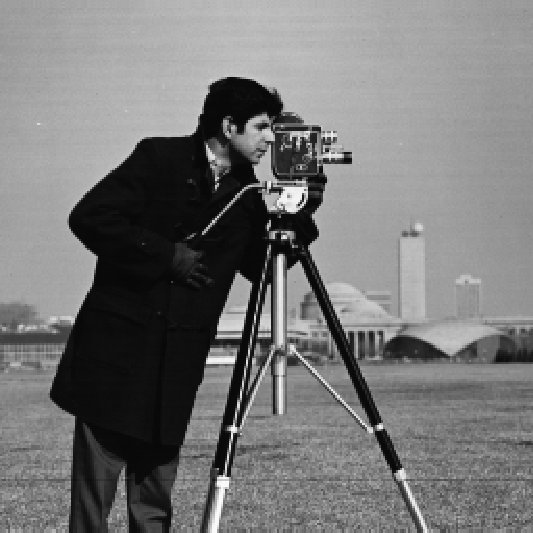
\includegraphics[width=0.8\columnwidth]{figures/cameraman.pdf}
   \caption{The original, unblurred cameraman image.  To create the blurred image, the $\mathcal{R}$ is applied to the original image and Gaussian noise is added.}
   \label{fig:cameraman_original}
\end{figure}

Figure \ref{fig:cameraman_200_db1_sym} shows the deblurred image after 200 iterations of FISTA, a fast proximal gradient method, developed by Beck and Teboulle \cite{beck_2009}.  The wavelet synthesis operator $\mathcal{W}$ is taken to be a three-stage Haar discrete wavelet transform with symmetric boundary conditions.  In this case, the operator $\mathcal{W}$ is orthogonal, so $\mathcal{W}^\ast = \mathcal{W}^\dagger$, which is the three-stage wavelet reconstruction operation with symmetric boundary conditions.  So, coding up the adjoint transform is a simple matter of performing the analysis operation with suitable boundary conditions.

\begin{figure}
   \centering
   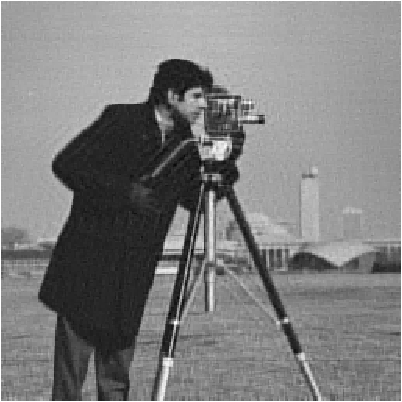
\includegraphics[width=0.8\columnwidth]{figures/cameraman_rec_200_db1_sym_trim.pdf}
   \caption{Deblurred image after 200 iterations of FISTA with $\mathcal{W}$ a three-stage Haar transform with symmetric boundary conditions.}
   \label{fig:cameraman_200_db1_sym}
\end{figure}


\subsection{The adjoint for biorthogonal wavelets}
For biorthogonal wavelets, we no longer have $\mathcal{W}^\ast=\mathcal{W}^\dagger$.  Since we have relaxed ourselves to biorthogonal wavelets, it is perhaps too much to ask that the adjoint of the primal wavelet synthesis operator involves only the primal wavelets.  Let us recall briefly the pertinent aspects of frames of Hilbert spaces.  These facts are described in more detail in \cite{mallat_2009}.\\

Let $\mathcal{H}$ be a Hilbert space and take $f\in\mathcal{H}$ to be an arbitrary vector in the Hilbert space.  Let $\{\phi_n\}_{n\in\Gamma}$, where $\Gamma$ is an index set, be a set of vectors in $\mathcal{H}$.  The set of vectors $\{\phi_n\}_{n\in\Gamma}$ is called a frame of $\mathcal{H}$ if there exists constants $B\ge A > 0$ such that

\[ \forall f\in \mathcal{H}, \quad A\|f\|^2 \le \sum_{n\in\Gamma} |\langle f,\phi_n\rangle|^2\le B \|f\|^2. \] 

\noindent If the set $\{\phi_n\}_{n\in\Gamma}$ is a frame and is linearly independent, we call it a Riesz basis.\\

We assume henceforth that the set $\{\phi_n\}_{n\in\Gamma}$ is a frame of $\mathcal{H}$ with bounds $B\ge A > 0$.  We can define the frame analysis operator $\Phi$ via

\[ \forall n\in \Gamma,\quad \Phi f[n] = \langle f,\phi_n\rangle. \] 

\noindent The frame analysis operator computes the expansion coefficients of $f$ in the frame $\{\phi_n\}_{n\in\Gamma}$.  The frame synthesis operator is $\Phi^\ast$, and constructs a vector in $\mathcal{H}$ given expansion coefficients.  Since $\{\phi_n\}_{n\in\Gamma}$ is assumed to be a frame, $\Phi^\ast\Phi$ is invertible, and we may define the Moore-Penrose pseudoinverse $\Phi^\dagger$, which implements reconstruction, as $\Phi^\dagger = \left(\Phi^\ast\Phi\right)^{-1}\Phi$.\\

Reconstruction with the pseudoinverse of the frame operator can be thought of as synthesis with a dual frame.  The dual frame analysis operator and dual frame vectors are defined via

\[ \forall n\in \Gamma, \quad \tilde{\Phi}f[n] = \langle f,\tilde{\phi}_n\rangle, \quad \text{where } \tilde{\phi}_n = \left(\Phi^\ast\Phi\right)^{-1}\phi_n. \] 

\noindent Then the dual frame synthesis operator satisfied $\tilde{\Phi}^\ast = \Phi^\dagger$.  Notice that we also have $\Phi^\ast = \tilde{\Phi}^\dagger$; this relation provides the basic idea for computing the adjoint of the discrete wavelet synthesis operator $\mathcal{W}$.  Ignoring boundary effects and selecting the biorthogonal wavelets so that $\Phi^\dagger=\mathcal{W}$, we have the following:

\begin{align*}
   \mathcal{W}^\ast &= \left(\Phi^\dagger\right)^\ast = \left(\left(\Phi^\ast\Phi\right)^{-1}\Phi^\ast\right)^\ast = \Phi\left(\Phi^\ast\Phi\right)^{-1}\\ 
                    &= \left(\Phi^\ast\right)^\dagger = \left(\tilde{\Phi}^\dagger\right)^\dagger\\
                    &= \tilde{\Phi},
\end{align*}

\noindent where we have used various properties of the pseudoinverse.  Thus, ignoring boundary conditions, the adjoint of wavelet synthesis is dual wavelet analysis!  Note that in the case of orthogonal wavelets, $\Phi^\ast\Phi$ is the identity, the dual frame is identically the primal frame, and ${\mathcal{W}^\ast = \tilde{\Phi}=\Phi=\mathcal{W}^\dagger}$, exactly as before.\\

It now remains to include boundary conditions.  A standard method for imposing boundary conditions on finite, discrete signals is to extend the signal to match those boundary conditions and perform the wavelet operations on the extended signal, assuming zero boundary conditions for the extended signal; this is the approach used in {\sc matlab}'s Wavelet Toolbox \cite{matlab_wt_2015}.  If we let $\mathcal{E}$ be the extension operator and $\mathcal{W}^\dagger_\text{zpd}$ be the wavelet analysis operator for extended signals under zero boundary conditions, we can write wavelet analysis as 
%TODO motivate why we use W_zpd better

\[ \mathcal{W}^\dagger = \mathcal{W}^\dagger_\text{zpd}\mathcal{E}. \] 

\noindent This separation of signal extension and wavelet operations provides a nice framework for determining the adjoint:

\[ \mathcal{W} = \mathcal{E}^\dagger\mathcal{W}_\text{zpd}, \quad \mathcal{W}^\ast = \mathcal{W}^\ast_\text{zpd}(\mathcal{E}^\dagger)^\ast. \] 

Consider a signal $y[n]$, $n=0,...,N-1$.  Let $L_p$ be the length of the wavelet analysis filters (one can zero-padd a shorter filter to length $L_p$).  The double sided zero-padded extension of $y[n]$ puts $L_p-1$ zeros on each end of the signal:
\[ \underbrace{0, ..., 0}_{L_p-1}, y[0], ..., y[N-1], \underbrace{0, ..., 0}_{L_p-1}. \]

\noindent We can write down the linear operator $\mathcal{E}_\text{zpd}$ as a matrix that performs this operation on $y[n]$.

\[ \mathcal{E}_\text{zpd} = \begin{bmatrix} 0_{(L_p-1)\times N}\\ I_{N\times N}\\ 0_{(L_p-1)\times N}\end{bmatrix} = \begin{bmatrix} 0 & 0 & \cdots & 0 & 0\\ \vdots & \vdots &\ddots & \vdots & \vdots\\ 0 & 0 & \cdots & 0 & 0\\[0.5em] 1 & 0 & \cdots & 0 & 0\\ 0 & 1 & \cdots & 0 & 0\\ \vdots & \vdots & \ddots & \vdots & \vdots\\ 0 & 0 & \cdots & 1 & 0\\ 0 & 0 & \cdots & 0 & 1\\[0.5em] 0 & 0 & \cdots & 0 & 0\\ \vdots & \vdots & \ddots & \vdots & \vdots\\ 0 & 0 & \cdots & 0 & 0\end{bmatrix}. \] 

\noindent Once we have this explicit form of $\mathcal{E}_\text{zpd}$, we can find the adjoint of its pseudoinverse.  In this case we have that $\left(\mathcal{E}_\text{zpd}^\dagger\right)^\ast = \mathcal{E}_\text{zpd}$.  Although the zero-padded extension is simple to work with, it is not usually a reasonable extension mode for practical applications.  A better extension mode is the half-point symmetric extension, which is the default extension mode in {\sc matlab}'s Wavelet Toolbox \cite{matlab_wt_2015}.\\

The double sided half-point symmetric extension reflects the signal about its boundaries in the following manner:

\[ \underbrace{y[L_p-1], ..., y[0]}_\text{Left extension}, y[0], ..., y[N-1], \underbrace{y[N-1], ..., y[N+L_p-2]}_\text{Right extension}. \] 

\noindent As in the zero-padded case, we can readily form a matrix that performs this operation on $y[n]$.

\[ \mathcal{E}_\text{sym} = \begin{bmatrix} & & \iddots & & &\\ & 1 &&&&\\ 1&&&&&\\1&&&&\\&1&&&&\\&&\ddots&&&\\&&&1&\\&&&&1\\&&&&1\\&&&1&\\&&\iddots&&\end{bmatrix}. \]

\noindent The adjoint of the pseudoinverse can be computed in closed form and essentially amounts to rescaling the nonzero entries of $\mathcal{E}_\text{sym}$.  Assuming $N > 2(L_p-1)$, which usually occurs in practice, the adjoint of the  pseudoinverse of $\mathcal{E}_\text{sym}$ is 

\[ \left(\mathcal{E}_\text{sym}^\dagger\right)^\ast = \begin{bmatrix} & \iddots \\ 1/2&&&&&\\1/2&&&&\\&\ddots&&&&&&\\&&1/2&\\&&&1\\&&&&\ddots\\&&&&&1\\&&&&&&1/2\\&&&&&&&\ddots\\&&&&&&&&1/2\\&&&&&&&&1/2\\&&&&&&&\iddots\\\end{bmatrix}. \]

\noindent If $N \le 2(L_p-1)$, the form of the pseudoinverse is slightly different, with some of the $1/2$ terms becoming $1/3$; both cases are considered in our implementation.


\begin{figure}
   \centering
   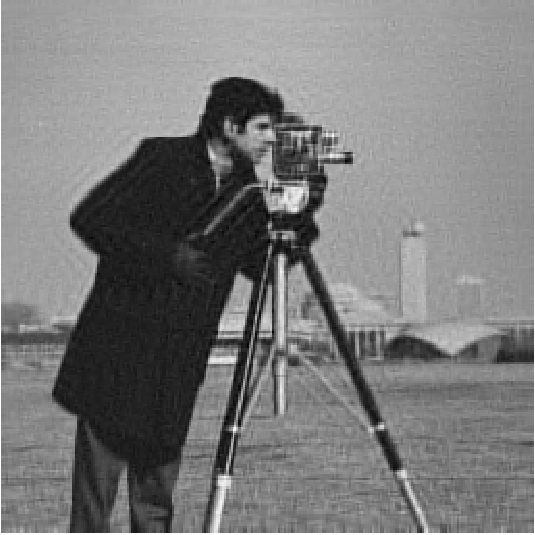
\includegraphics[width=0.8\columnwidth]{{figures/cameraman_rec_200_bior4.4_sym_trim}.pdf}
   \caption{Deblurred image after 200 iterations of FISTA with $\mathcal{W}$ a three-stage CDF 9/7 transform with symmetric boundary conditions.}
   \label{fig:cameraman_200_bior4.4_sym}
\end{figure}

Figure \ref{fig:cameraman_200_bior4.4_sym} shows the deblurred cameraman image after 200 iterations of FISTA using a three-stage CDF 9/7 transform with symmetric boundary conditions.
%TODO comment on sparsity levels of db1 vs bior4.4?  That's not really a fair comparison...



%TODO include this section too (but beware: it's old!)
%TODO briefly mention P. Combettes one theorem regarding unequivalence of analysis and synthesis formulation
%     for nonorthogonal transforms (and how the proximal mapping plays into why).
%\subsection{Analysis Formulation}
%We note here that there is an alternative formulation of the image deblurring problem.  The formulation (\ref{eq:syn_problem}), where $x$ is a vector of wavelet coefficients, is called the synthesis form.  We can also consider the problem in analysis form:
%
%\begin{equation}
%\label{eq:ana_form}
%\min_y \|\mathcal{R}y-b\|_2^2 + \lambda \|\mathcal{W}^\dagger y\|_1.
%\end{equation}
%
%\noindent We use $\mathcal{W}^\dagger$ to denote the Moore-Penrose pseudoinverse of $\mathcal{W}$; this is the standard operation of wavelet analysis.  In the analysis form, the optimization variable $y$ is an image.  An optimal solution $y^\ast$ should be a good approximation of the original, sharp image.\\
%
%If the wavelet synthesis operator is orthogonal, so that ${\mathcal{W}^\ast=\mathcal{W}^\dagger=\mathcal{W}^{-1}}$, we then have ${x=\mathcal{W}^{-1}y}$.  Moreover, the synthesis and analysis formulations are equivalent, in the sense that an optimal solution of one formulation is readily obtained from an optimal solution of the other.\\

%Wavelet software packages (e.g. \cite{matlab_wt_2015}) implement fast wavelet analysis and synthesis operators, which we can apply to 

% ]]]

\section{Example 2: Blind Channel Estimation}
% [[[
Another application where an interesting adjoint is involved in the gradient computation is in blind channel estimation.  In blind channel estimation, a single source sends an unknown signal over multiple channels with unknown response.  Observers collect the output of each channel and collectively attempt to determine the source signal and the channel impulse response from each channel.  Let $s$ be the unknown source signal and $h_i$ the channel impulse response of the $i$th channel.  Then the output of the $i$th channel is

\[ x_i = h_i\ast s. \] 

\noindent In this form, we must solve a multitude of nonlinear equations in the components of $s$ and each $h_i$.  



% ]]]

% References
% copied from ../notes/adjoint_wavelet_notes.bbl
% [[[
\documentclass{article}
%\documentclass[draft]{article}
% Functions, packages, etc.
%[[[
\usepackage{amsmath}
\usepackage{amsfonts}
\usepackage{amssymb}
\usepackage{amsthm}
\usepackage{array}
\setcounter{MaxMatrixCols}{20}

\usepackage{mathdots} % for \iddots

\usepackage{graphicx}
%\usepackage{subfig}
\usepackage[labelfont=bf]{caption}
%\usepackage[labelfont=bf]{subcaption}
\usepackage[top=1in, bottom=1in, left=1in, right=1in]{geometry}
\pagenumbering{arabic}
\usepackage{hyperref}
\usepackage{enumerate}
%\numberwithin{equation}{section}
%\usepackage{soul} % for \ul - a ``better'' underlining command

%\usepackage{colortbl} % for coloring \multicolumn (tabular in general, I think)
% For \rowcolor
%\definecolor{table_header}{gray}{0.5}
%\definecolor{table_data}{gray}{0.85}


%% Inserting code and syntax highlighting
% [[[
\usepackage{listings} % like verbatim, but allows for syntax highlighting and more
\usepackage{color} % colors
\usepackage[usenames,dvipsnames]{xcolor}% More colors
\usepackage{caption} % captions
\DeclareCaptionFont{white}{\color{white}}
\DeclareCaptionFormat{listing}{\colorbox{gray}{\parbox{\textwidth}{#1#2#3}}}
\captionsetup[lstlisting]{format=listing,labelfont=white,textfont=white}
\usepackage{framed} % put a frame around things

% define some custom colors
\definecolor{dkgreen}{rgb}{0,0.6,0}
\definecolor{lgreen}{rgb}{0.25,1,0}
\definecolor{purple}{rgb}{0.35,0.02,0.48}

% Some changes to MATLAB/GNU Octave language in listings
\lstset{frame=tbrl,
    language=Matlab,
    aboveskip=3mm,
    belowskip=3mm,
    belowcaptionskip=3mm,
    showstringspaces=false,
    columns=flexible,
    basicstyle={\small\ttfamily\color{black}},
    numbers=left,
    numberstyle=\tiny\color{purple},
    keywordstyle=\color{dkgreen},
    commentstyle=\color{red},
    stringstyle=\color{purple},
    breaklines=true,
    breakatwhitespace=true,
    tabsize=4,
    rulecolor=\color{black},
    morekeywords={string,fstream}
}
% ]]]


%My Functions
\newcommand{\diff}[2]{\dfrac{d #1}{d #2}}
\newcommand{\diffn}[3]{\dfrac{d^{#3} #1}{d {#2}^{#3}}}
\newcommand{\pdiff}[2]{\dfrac{\partial #1}{\partial #2}}
\newcommand{\pdiffn}[3]{\dfrac{\partial^{#3} #1}{\partial {#2}^{#3}}}
\newcommand{\drm}{\mathrm{d}}
\newcommand{\problemline}{\rule{\textwidth}{0.25mm}}
\newcommand{\problem}[1]{\problemline\\#1\\\problemline\vspace{10pt}}
\newcommand{\reals}{\mathbb{R}}
\newcommand{\qline}[2]{\qbezier(#1)(#1)(#2)}
\newcommand{\abox}[1]{\begin{center}\fbox{#1}\end{center}}
\newcommand{\lie}{\mathcal{L}}
\newcommand{\defeq}{\stackrel{\operatorname{def}}{=}}


% AMS theorem stuff
% [[[
\newtheoremstyle{mystuff}{}{}{\itshape}{}{\bfseries}{:}{.5em}{}
\theoremstyle{mystuff}
\newtheorem{definition}{Definition}[section]
\newtheorem*{definition*}{Definition}
\newtheorem{theorem}{Theorem}[section]
\newtheorem*{theorem*}{Theorem}
\newtheorem{lemma}{Lemma}[section]
\newtheorem*{lemma*}{Lemma}
\newtheorem*{proposition*}{Proposition}
\newtheorem{corallary}{Corallary}
\newtheorem*{remark}{Remark}

\newtheoremstyle{myexample}{}{}{}{}{\bfseries}{:}{.5em}{}
\theoremstyle{myexample}
\newtheorem*{example*}{Example}


% Stolen from http://tex.stackexchange.com/questions/8089/changing-style-of-proof
\makeatletter \renewenvironment{proof}[1][\proofname] {\par\pushQED{\qed}\itshape\topsep6\p@\@plus6\p@\relax\trivlist\item[\hskip\labelsep\bfseries#1\@addpunct{:}]\ignorespaces}{\popQED\endtrivlist\@endpefalse} \makeatother

% Stolen from http://tex.stackexchange.com/questions/12913/customizing-theorem-name
\newtheoremstyle{named}{}{}{\itshape}{}{\bfseries}{:}{.5em}{\thmnote{#3's }#1}
\theoremstyle{named}
\newtheorem*{namedtheorem}{Theorem}
% ]]]

%]]]

% Output Control Variables
\def\true{1}
\def\false{0}
\def\figures{1}
\def\tables{1}
%\usepackage{showkeys}

\title{Adjoint Wavelet}
%\date{}
\author{James Folberth}


\begin{document}
\maketitle
\tableofcontents

\section{Introduction}
% [[[

The adjoint (transpose for real wavelets) of wavelet analysis operators appear in some image deblurring problems \cite{beck_2009}. As an example, let $R$ be a known blurring operator, $W$ a wavelet analysis operator, and $b$ an image blurred under the action of $R$. Since we expect images to have sparse wavelet coefficients, the following problem formulation is reasonable:

\[ \min_x \|RWx-b\|_2^2 + \lambda \|x\|_1. \] 

\noindent The gradient of the first term is $2W^*R^*(RWx-b)$. One can use this with a (fast) proximal gradient method (e.g. FISTA \cite{beck_2009}). We can compute the action of $R$ and $R^*$ efficiently in the Fourier domain. However, wavelet toolboxes do not provide an efficient means to compute $W^*$, as it is not a standard operation. The standard operations are $W$ and $W^\dagger$, the pseudoinverse.\\

If the wavelet analysis operator is orthogonal, we can reformulate the problem exactly, so we no longer need $W^*$ (\cite{combettes_2007}, Proposition 11):

\[ \min_y \|Ry-b\|_2^2 + \lambda \|W^\dagger y\|_1. \] 

\noindent Additionally, we know that $W^*=W^\dagger$, so we could solve the original problem.\\

For non-orthogonal wavelet operators (e.g. CDF wavelets, which are used in the JPEG 2000 standard \cite{skodras_2001}), the reformulation is not exact.  We would like to compute the action of $W^*$ in $\mathcal{O}(N)$ operations, which would facilitate the efficient solution of the original problem.\\

Another approach is to compute the gradient $2W^*R^*(RWx-b)$ using automatic differentiation.  Initial experiments suggest that this does not scale well with image size, and therefore is not a viable approach.\\

% ]]]

\section{Adjoint wavelet}
% [[[

\subsection{Frames}
% [[[
Let $\mathcal{H}$ be a Hilbert space.  Let the inner product be linear in its first argument.  An idea is to try to recover a signal $f\in\mathcal{H}$ from its inner products with a family of vectors $\{\phi_n\}_{n\in\Gamma}$, where $\Gamma$ is an index set.  Frames are used to provide conditions under which this recovery is possible.\\

\begin{definition*}[5.1, Mallat]
   The sequence $\{\phi_n\}_{n\in\Gamma}$ is a \textbf{frame} of $\mathcal{H}$ if there exist constants $B\ge A\ge 0$ such that 

   \[ \forall f\in\mathcal{H}, \quad A\|f\|^2 \le \sum_{n\in\Gamma} |\langle f, \phi_n\rangle|^2 \le B\|f\|^2. \] 

   \noindent When $A=B$, the frame is said to be \textbf{tight}.  If the $\{\phi_n\}_{n\in\Gamma}$ are linearly independent then the frame is not redundant and is called a \textbf{Riesz basis}.\\
\end{definition*}

\noindent If the frame condition is satisfied, we may define a so-called \textbf{frame analysis operator} $\Phi$:

\[ \forall n\in \Gamma, \quad \Phi f[n] = \langle f, \phi_n\rangle. \] 

\noindent Let $\ell^2(\Gamma)$ be the space of finite energy coefficients:

\[ \ell^2(\Gamma) = \{a \,:\, \|a\|^2 = \sum_{n\in\Gamma} |a[n]|^2 < \infty \}. \] 

\noindent The adjoint $\Phi^\ast$ is defined over $\ell^2(\Gamma)$ as usual:

\[ \langle \Phi^\ast a, f\rangle = \langle a, \Phi f\rangle = \sum_{n\in\Gamma} a[n]\langle f, \phi_n\rangle^\ast. \] 

\noindent It is therefore the synthesis operator

\[ \Phi^\ast a = \sum_{n\in \Gamma} a[n]\phi_n. \] 

The reconstruction of $f$ from its frame coefficients $\Phi f[n]$ is computed with the Moore-Penrose pseudoinverse $\Phi^\dagger$.


\begin{theorem*}[5.4, Mallat]
   If $\Phi$ is a frame operator, then $\Phi^\ast\Phi$ is invertible and the pseudo inverse satisfies

   \[ \Phi^\dagger = (\Phi^\ast\Phi)^{-1}\Phi^\ast. \] 
\end{theorem*}

\noindent The pseudoinverse handles reconstruction through synthesis in a dual frame.  This is the central result that guides us in the construction of the adjoint wavelet analysis operator.

\begin{theorem*}[5.5, Mallat]
   Let $\{\phi_n\}_{n\in\Gamma}$ be a frame with bounds $0<A\le B$.  The dual operator defined via

   \[ \forall n\in \Gamma, \quad \widetilde{\Phi} f[n] = \langle f, \tilde{\phi}_n\rangle, \quad \tilde{\phi}_n = (\Phi^\ast\Phi)^{-1} \phi_n \] 

   \noindent satisfies $\widetilde{\Phi}^\ast = \Phi^\dagger$, and thus

   \[ f = \sum_{n\in\Gamma} \langle f, \phi_n\rangle \tilde{\phi}_n = \sum_{n\in\Gamma} \langle f, \tilde{\phi}_n\rangle \phi_n. \] 

   \noindent It defines a dual frame as

   \[ \forall f\in\mathcal{H}, \quad \frac{1}{B}\|f\|^2 \le \sum_{n\in\Gamma} |\langle f, \tilde{\phi}_n\rangle|^2 \le \dfrac{1}{A} \|f\|^2. \] 

   \noindent If the frame is tight (i.e., $A=B$), then $\tilde{\phi}_n=A^{-1}\phi_n$.
\end{theorem*}

We can now specialize the results given above to the problem at hand: compute the action of $W^\ast$, where $W$ is a (multistage) wavelet analysis operator.  From Theorem 5.5 of Mallat (cited above), we know that $\widetilde{\Phi}^\ast = \Phi^\dagger$.  Do we have $\Phi^\ast = \widetilde{\Phi}^\dagger$?  If $\widetilde{W}$ is the dual wavelet analysis operator, do we have $W^\ast = \widetilde{W}^\dagger$, even for finite length signals?  It turns out that with slight modification to the way one handles boundary conditions, the answer is yes!\\

The action of $W$ is analysis with the (primal) wavelet.  For orthogonal wavelets, the action of $\widetilde{W}^\dagger$ is reconstruction with the (primal) wavelet.  For biorthogonal wavelets, the action of $\widetilde{W}^\dagger$ is reconstruction with the dual (reverse) wavelet.\\

% ]]]

\subsection{Adjoint wavelet for finite length signals}
% [[[
A lot of the wavelet theory is done for infinite length signals.  In applications, however, we often deal with finite signals.  In the process of computing wavelet coefficients, we must make assumptions about the behavior of the signal past the boundaries.  One common method of treating the boundaries of finite signals is to extend the signal at the boundaries.  Common extension methods assume the signal is zero outside the boundary, the signal is periodic, or that the signal is symmetric about the boundaries.  {\sc matlab}'s default extension method is the half-point symmetric extension \cite{matlab_wt_2015, strang_1996}.\\

We can separate the various signal extension methods (each a linear operation) from the computation of the wavelet coefficients.  A wavelet operator $W$ can be factored, in a loose sense, as

\[ W = W_\text{zpd}E, \] 

\noindent where $W_\text{zpd}$ is the wavelet analysis under zero-padded boundary conditions and $E$ is the preferred signal extension operator.  Thus, the action of $W$ on a signal $x$ occurs in two stages: first, extend the signal $x$ under the action of $E$; second, compute the wavelet coefficients of the extended signal assuming the extended signal has zero-padded boundary conditions.\\

We noticed that $W^\ast_{\text{zpd}}=\widetilde{W}_{\text{zpd}}^\dagger$.  This did not occur for other, more appropriate, extension modes.  However, we do have

\[ W^\ast = E^\ast W^\ast_{\text{zpd}} = E^\ast \widetilde{W}^\dagger_\text{zpd}. \] 

\noindent One can readily find the adjoint of the extension operator $E$ (as we will show in the next few subsections).  Applying $\widetilde{W}^\dagger_\text{zpd}$ is a standard operation in {\sc matlab}'s Wavelet Toolbox.\\

% ]]]

\subsection{Adjoint extension - zero-padded}
% [[[
We will first handle the case of a one-dimensional signal, $x$, with entries $x[0], ..., x[N-1]$.  Let $L_p$ be the length of the wavelet analysis filters.  We extend the signal to have $L_p-1$ zeros on both the right and left sides.

\[ \underbrace{0, ..., 0}_{L_p-1}, x[0], ..., x[N-1], \underbrace{0, ..., 0}_{L_p-1} \]

\noindent We can represent this extension $E$ as a matrix, which will act on the vector $x$:

\[ E = \begin{bmatrix} 0_{(L_p-1)\times N}\\ I_{N\times N}\\ 0_{(L_p-1)\times N}\end{bmatrix} = \begin{bmatrix} 0 & 0 & \cdots & 0 & 0\\ \vdots & \vdots &\ddots & \vdots & \vdots\\ 0 & 0 & \cdots & 0 & 0\\[0.5em] 1 & 0 & \cdots & 0 & 0\\ 0 & 1 & \cdots & 0 & 0\\ \vdots & \vdots & \ddots & \vdots & \vdots\\ 0 & 0 & \cdots & 1 & 0\\ 0 & 0 & \cdots & 0 & 1\\[0.5em] 0 & 0 & \cdots & 0 & 0\\ \vdots & \vdots & \ddots & \vdots & \vdots\\ 0 & 0 & \cdots & 0 & 0\end{bmatrix} \] 

\noindent We then have

\[ E^\ast = \begin{bmatrix} 0_{N\times (L_p-1)} & I_{N\times N} & 0_{N\times (L_p-1)} \end{bmatrix}. \] 

\noindent The action of $E^\ast$ on a vector is simply cutting off $L_p-1$ entries from the left and right sides.\\

% ]]]

\subsection{Adjoint extension - half-point symmetric}
% [[[
The half-point symmetric extension is discussed in \cite{strang_1996}.  We extend the signal $x$ by reflecting $L_p-1$ entries across the left and right boundaries, with symmetry about the points $1/2$ and $N-1/2$ (hence the name half-point symmetry).  The extended signal has entries the following entries.

\[ \underbrace{x[L_p-1], ..., x[0]}_\text{Left extension}, x[0], ..., x[N-1], \underbrace{x[N-1], ..., x[N+L_p-2]}_\text{Right extension}  \] 

\noindent We can represent this extension $E$ as a matrix, which will act on the vector $x$:

\[ E = \begin{bmatrix} & & \iddots & & &\\ & 1 &&&&\\ 1&&&&&\\1&&&&\\&1&&&&\\&&\ddots&&&\\&&&1&\\&&&&1\\&&&&1\\&&&1&\\&&\iddots&&\end{bmatrix} \] 

The adjoint is

\[ E^\ast = \begin{bmatrix}
            &&1&1&&&&&&&\\
            &1&&&1&&&&&&\\
            \iddots&&&&&\ddots&&&&&\iddots\\
            &&&&&&1&&&1&\\
            &&&&&&&1&1&&
            \end{bmatrix}. \] 

\noindent The action of the adjoint is to fold and sum the length $L_p-1$ ends of the signal back onto the corresponding portion of the original signal.\\

For the extension of a matrix, the extension operator acts in a Kronecker product type fashion.  Below is the relevant portion of \verb|extension_adjoint_2d.m|.

\begin{lstlisting}[language=matlab]
% this feels like a Kronecker product
% do the first dimension update (fold and add, like in 1d)
x = xe(le+1:le+lX(1), :);
x(1:le, :) = x(1:le, :) + xe(le:-1:1, :);
x(end-le+1:end, :) = x(end-le+1:end, :) + xe(end:-1:end-le+1, :);

% then do the second dimension update (fold and add)
xe = x; % alias
x = x(:, le+1:le+lX(2));
x(:, 1:le) = x(:, 1:le) + xe(:, le:-1:1);
x(:, end-le+1:end) = x(:, end-le+1:end) + xe(:, end:-1:end-le+1);
\end{lstlisting}


% ]]]

% ]]]


\section{How close is $W^\ast W$ to $I$?}
% [[[
%TODO

\begin{figure}[ht!]
   \centering
   \includegraphics[width=\textwidth]{figures/WTW_db2_3_levels_zpd_trim.pdf}
   \caption*{$W^*W$, db2, 3 levels, zero-padded BCs.}
\end{figure}

\begin{figure}[ht!]
   \centering
   \includegraphics[width=\textwidth]{figures/WTW_db2_3_levels_sym_trim.pdf}
   \caption*{$W^*W$, db2, 3 levels, half-point symmetric BCs.}
\end{figure}

\begin{figure}[ht!]
   \centering
   \includegraphics[width=\textwidth]{{figures/WTW_bior4.4_3_levels_zpd_trim}.pdf}
   \caption*{$W^*W$, bior4.4, 3 levels, zero-padded BCs.}
\end{figure}

\begin{figure}[ht!]
   \centering
   \includegraphics[width=\textwidth]{{figures/WTW_bior4.4_3_levels_sym_trim}.pdf}
   \caption*{$W^*W$, bior4.4, 3 levels, half-point symmetric BCs.}
\end{figure}

% ]]]


\cite{mallat_2009}
\cite{strang_1996}
\cite{beck_2009}
\cite{hansen_2006}
\cite{becker_2011}

\clearpage
\bibliographystyle{IEEEtran}
\bibliography{adjoint_wavelet.bib}

\end{document}

% vim: set spell:
% vim: foldmarker=[[[,]]]

% ]]]

% if you will not have a photo at all:
\begin{IEEEbiographynophoto}{James Folberth}
Biography text here.
\end{IEEEbiographynophoto}

% if you will not have a photo at all:
\begin{IEEEbiographynophoto}{Stephen Becker}
Biography text here.
\end{IEEEbiographynophoto}

\end{document}

% vim: set spell:
% vim: foldmarker=[[[,]]]
